\documentclass[11pt]{article}
\usepackage{amsmath}
\usepackage{graphicx}
\usepackage{color}
\usepackage{longtable}
\usepackage{tabu} %% text tables
%%\usepackage[linktocpage=true]{hyperref} %% links to numbers instead of sections
\usepackage{hyperref}
%%\usepackage{url}
\usepackage{geometry}
\geometry{left=1.5cm,right=1.5cm,top=1.5cm,bottom=1.5cm}
\graphicspath{{./images/}}
\usepackage{amsmath}
\usepackage{amssymb}
\usepackage{calc}
\usepackage{ifthen}
\usepackage{tikz}
\usepackage{svg}
\usepackage{float}
%%\usepackage{cite}
%%\usepackage{notoccite}
\usepackage[backend=bibtex,sorting=none]{biblatex}
\addbibresource{seedom.bib}
\renewcommand*\rmdefault{ppl}
\setlength{\fboxsep}{10pt}
\setlength{\fboxrule}{0.5pt}

\begin{document}

\title{%
\begin{center}

\includegraphics[width=0.8\textwidth]{seedom6.pdf}
\end{center}
\large An Ether-raiser for Charities and Their Supporters \\[1mm]}
\author{Team Palm Tree}
\date{\today}
\maketitle

\begin{abstract}

There isn't an efficient, transparent, and trustless system that rewards philanthropists of any stature, impactful charities, and the members of society these individuals better. Fundraisers in any form take time to put together, lack full transparency, and foster only a transient connection to the cause. Campaigns to promote fundraisers require significant effort, especially when potential donors lack proximity to the issue.

Seedom is a platform that allows anyone to contribute ether for distribution to legitimate charities and a participant in Seedom's trustless smart contract. Bimonthly, a new active and demanding charity will be chosen to receive the majority of funds raised through our smart contract. Most of the remaining portion will go to one of the supporters through a selection process crowd-sourced by the participants. A small percentage will be taken by the Seedom team as an administration fee to continuously improve the platform over time and extensively promote each charity.

\end{abstract}
\pagebreak

\tableofcontents
\pagebreak

\section{Introduction}

Seedom is an Ethereum decentralized application for raising awareness and ether for charities in need while rewarding a single participant for their contribution and support. The selection of the winning participant is crowd-sourced from the participants and the selected charity. Funds raised will be distributed according to Table \ref{tab:fundSplitPercentages}. Administration fees cover our expenses in four operational areas.

\begin{itemize}
\item{\textbf{Staff} team members, which include the president, founders, software developers, and the marketing team}
\item{\textbf{Legal} representation to protect all forms of private ether-raising rights internationally}
\item{\textbf{Audits} continual security and financial audits as changes to the contract and our organization are made}
\item{\textbf{Events} additional physical ether-raisers to further raise money for and promote charities}
\end{itemize}

\begin{table}[H]
\begin{center}
\begin{tabular}{| l | l | l |}
\hline
\textbf{Charity} & \textbf{Winner} & \textbf{Seedom} \\ \hline
60\% & 35\%  & 5\% \\ \hline
\end{tabular}
\caption{Fund split percentages}
\label{tab:fundSplitPercentages}
\end{center}
\end{table}

\subsection{Charity Selection}

Well before an ether-raiser begins, the Seedom team will accept suggestions from the global community. The Seedom team will have the discretion of charity selection for the first release, identifying an organization that is legitimate, active, demanding, and cooperative, as described below. A future goal is to open up this selection process further to have it be community driven.

\begin{itemize}
\item{\textbf{Legitimate} the charity must be a non-profit with a proven record of benefiting the general public}
\item{\textbf{Active} the charity must be actively working on a cause}
\item{\textbf{Exacting} there should be an urgent or ongoing unresolved need by the charity for assistance}
\item{\textbf{Cooperative} the charity must be willing to work with the Seedom team}
\end{itemize}

\subsection{Combination of Qualities}

Seedom is the first ether-raiser and rewards platform with all of the following qualities.

\begin{itemize}
\item{\textbf{Philanthropic} a new charity will be chosen bimonthly}
\item{\textbf{Trustless} trust in the charity is all that is required}
\item{\textbf{Transparent} all contract transactions publicly visible and immutable}
\item{\textbf{Relevant} our team only works with legitimate charities working on focused causes that have an ongoing need for assistance}
\item{\textbf{Secure} security provided by the Ethereum platform itself and MetaMask}
\item{\textbf{Anonymous} a wallet is the only requirement}
\item{\textbf{Private} any identifying information given is purged after each ether-raiser}
\item{\textbf{Inclusive} anyone in the world can participate}
\item{\textbf{Affordable} everyone will be able to afford an entry}
\item{\textbf{Limitless} there is no limit to the number of obtainable entries}
\item{\textbf{Instantaneous} payouts to the charity and the winning participant are immediate after the ether-raiser ends}
\end{itemize}

\subsection{Seedom Trustlessness}

While the Seedom community relies on the administration team to choose legitimate, active, exacting, and cooperative charities twice a month, no further trust is required in our team. Once an ether-raiser has begun, the charity being supported by the community has complete control of the contract until the next ether-raiser begins. By handing control of the smart contract over to the charity, they function as the trusted third party. However, there is a cancellation routine open to the charity and the Seedom team, that will refund everyone their ether.

\subsection{Comparison to Other Fundraising Methods}

Many methods exist for raising funds for charities. Outside of direct donations, some of the most popular include crowdfunding, matching gifts, drives, sales, auctions, events, lotteries, and raffles. All of these methods lack many of our combined qualities.

\subsubsection{Crowdfunding}

Crowdfunding is one of the best ways to raise funds for a charity or cause. Unfortunately, most of the popular fundraising platforms are not on Ethereum and therefore receive none of the many benefits native to the platform. When using a centralized website, such as GoFundMe, one is relying on them as to move funds from donors to a charity. Without trustless transaction transparency, it is impossible to know if these contributions ever made it to the cause. Moreover, many crowdfunding companies charge 8+\% fees for any donation, which includes a hefty payment processing fee. With this reliance on payment processors, GoFundMe is only available in a handful of counties.

\subsubsection{Matching, Drives, Sales, and Auctions}

Matching, drives, sales, and auctions are also useful fundraising vehicles. Donation matching requires one to work for or know a company that offers this perk. Donation drives may involve an intermediary that converts non-monetary donations into the monetary type. Sales of items require the overhead of procuring items to sell in addition to the resale activity. Auctions items must be solicited, hopefully for free, and then sold for donation funds. Because of the various requirements and overheads involved with each of these techniques, the timeliness and relevancy of the donations are significant concerns; with intermediaries involved, trust and transparency are paramount yet not easily demonstrated. Moreover, all three of these methods also lack global participation capability.

\subsubsection{Events}

Fundraising events are social gatherings that raise funds and awareness for a charity. Often overlooked, face to face communication is indispensable to furthering a cause. However, these gathers can get expensive when selecting a venue, hiring temporary staff, providing food, creating informative materials, etc. Seedom adopts this face-to-face approach at the end of each ether-raiser in the form of fundraising and volunteering events. At this point, the bulk of the funds are raised and distributed, making this final event valuable, but not necessary to the success of the overall ether-raiser.

\subsubsection{Lotteries \& Raffles}

Although Seedom is not a lottery and not a raffle, similar organizations exist worldwide, and all of them have administration fees for their existence. In the United States, nearly every state has a lottery, with a national average administration fee of 4.76\% according to the U.S. Census Bureau \cite{3}; however, this does not include commissions paid out to lottery ticket sellers, which equal this same percentage, on average \cite{4}. All expenses considered, 8-10\% of every lottery ticket sold in the U.S. goes towards the lottery process itself and not the winner(s) and beneficiaries.

\subsection{Similar Ethereum Projects}

Alice, Charitychain, Giveth, and Hypergive are other experimental non-profit Ethereum fundraising applications currently under development. Many of these systems go beyond fundraising and seek to control the internal operations of the non-profits funded. The first three allow donation refunds if the charity does not meet their promised goals promptly, however these goals might be defined. Seedom's less authoritarian approach embraces facilitation, freeing the charity to manage their internal operations while streamlining their fundraising efforts. This separation of concerns is necessary and maintains the charity's ability to improve their efforts in their way, outside of Seedom's control.

Hypergive creates a direct and secure funding connection between donators and homeless and hungry individuals globally. This channel is similar to one employed by an aid program run by the United Nations that delivered funds to 10,000 Syrian refugees using the Ethereum blockchain \cite{6}. Seedom will seek to partner with any organization working on these type of trustless end-to-end philanthropic delivery mechanisms as they are a fantastic use-case for the Ethereum platform. Additionally, the Seedom team will offer training services to the charities worked with to bring them up to speed on these emerging blockchain technologies.

\section{The Bimonthly Trustless Ether-raiser}

Seedom will kickoff a new ether-raiser for a new charity bimonthly, or roughly every two weeks, on the 1st and 15th of every month. Thirteen days is the span of the entire timeline due to February's 28 total days during standard years. Seedom will go on break on the 13th and 14th of every month in addition to the 29th until the end of any month long enough.

\begin{figure}[H]
\begin{center}
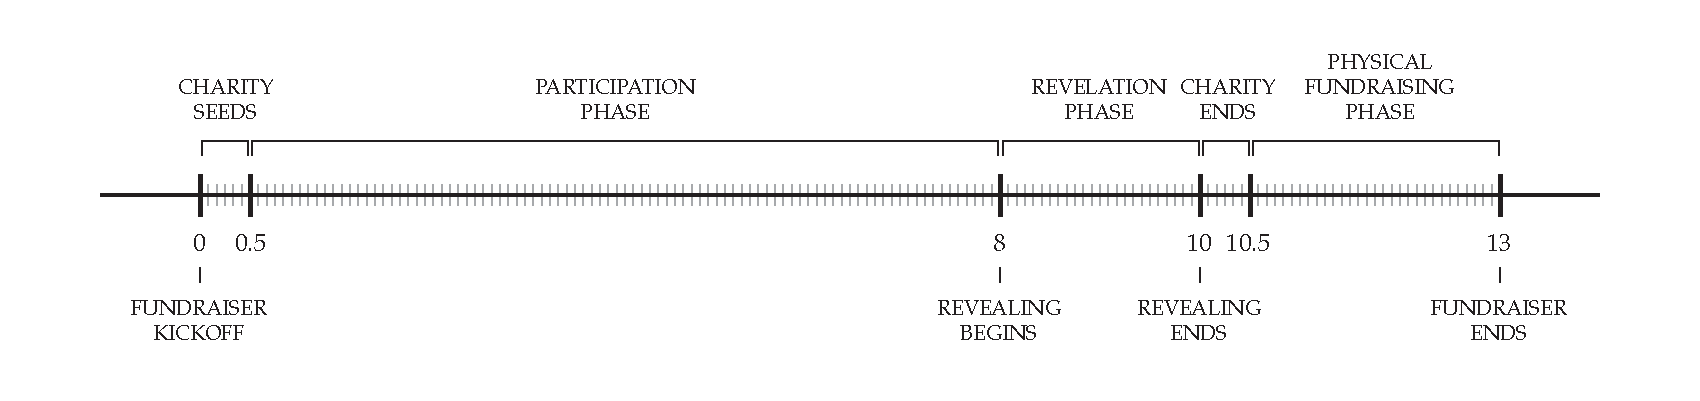
\includegraphics[width=1.0\textwidth]{etherraiserBimonthlyTimeline.pdf}
\caption{Ether-raiser bimonthly timeline}
\label{figure:etherraiserBimonthlyTimeline}
\end{center}
\end{figure}

\subsection{Ether-raiser Kickoff}
An ether-raiser begins with the Seedom team kicking it off through our smart contract by providing several parameters defined in Table \ref{tab:etherraiserKickoffParameters}.

\begin{table}[H]
\begin{center}
\begin{tabular}{| l | l | l |}
\hline
\textbf{Parameter} & \textbf{Data type} & \textbf{Description} \\ \hline
charity & address & the wallet address of the charity \\ \hline
charitySplit & uint256 & the \% of funds given to the charity \\ \hline
winnerSplit & uint256 & the \% of funds given to the winner \\ \hline
ownerSplit & uint256 & the \% of funds given to the owner \\ \hline
valuePerEntry & uint256 & unix timestamp of the start of revelation phase \\ \hline
revealTime & uint256 & unix timestamp of the end of revelation phase \\ \hline
expireTime & uint256 & unix timestamp of the expiration of the ether-raiser \\ \hline
\end{tabular}
\caption{Ether-raiser kickoff parameters}
\label{tab:etherraiserKickoffParameters}
\end{center}
\end{table}

\subsection{Charity Seeds}
Shortly after kickoff, the charity must create a 32-byte random number and hash it. The hashed random, the address of the charity's wallet, and the address of the active Seedom contract will be posted by the charity and Seedom through our respective social media accounts to guarantee their origin and authenticity. Any user can validate these pieces of data against the contract address state.

The charity will now seed the charity a 32-byte hash of it. Only the charity can provide this hashed number, and no one can participate for the remainder of the ether-raiser if not given. All hashed randoms are generated using the hashed random formula in Figure \ref{figure:hashedRandomNumberFormula}. The charity must safeguard their random number and not reveal it to anyone outside of their organization. It will be used later when the charity ends the ether-raiser. If the charity does not seed the ether-raiser before the revelation phase, the ether-raiser is inoperable, with all participants receiving refunds upon cancellation.

\begin{figure}[H]
\begin{center}
\fbox{$hashedRandomNumber = sha3_{keccak256}(randomNumber, ethereumAddress)$}
\caption{Hashed random number formula (randomNumber is 32 bytes, ethereumAddress is 20 bytes)}
\label{figure:hashedRandomNumberFormula}
\end{center}
\end{figure}

\subsection{Participation Phase}

After the charity has submitted their hashed random number, the ether-raiser is considered open, and anyone can now participate and send ether to the contract. Participation is a one-time activity, and prior, a user must create a personal 32-byte random number and hash it using the formula in Figure \ref{figure:hashedRandomNumberFormula}. The user must safeguard their random number and not reveal it to anyone else. It will be used during the revelation phase to confirm their participation in the ether-raiser, and during the end function, to uniquely identify the winning participant.

Each entry costs a fixed value determined by the Seedom team at kickoff. The cost of a single entry, including Ethereum transaction fees, will be globally affordable to allow those beneath the international poverty line of \$1.90 (USD) per day \cite{1} to participate, with a minimum entry being less than the ether equivalent of this amount. Each entry increases the likelihood that you will be selected by both the community and the charity to receive a split percentage of all of the ether contributed by the contract, similar to a raffle. The winner will be invited to participate in the physical ether-raiser event after charity end. Entries are non-refundable except after ether-raiser cancellation and need confirmation during the revelation phase for winner consideration. Partial entries are immediately refunded during participation or through additional funding afterward. The owner and the charity are never allowed to participate.

Along with the hashed random and any ether, a user can optionally associate their Ethereum address with a short alias and their email address. These three values are stored off-chain in Seedom's secure database servers and forgotten by the time the next ether-raiser begins to protect participant privacy and keep our system compliant of data privacy legislation, such as the European Union's General Data Protection Regulation (GDPR). For the first release, aliases are used to render a list of recent participants. The email address is only used to invite the community-chosen winning supporter to the physical ether-raiser during the last few days.

Ether can be sent along with participation requests to obtain initial entries, and more can be sent afterward through the fallback function for the same purpose. However, additional calls to the participate function will fail as participant hashed random numbers are immutable. There is no limit to the number of entries a participant can acquire, and the participant can check the number of entries they or any other participant has through the contract at any time.

\begin{figure}[H]
\begin{center}
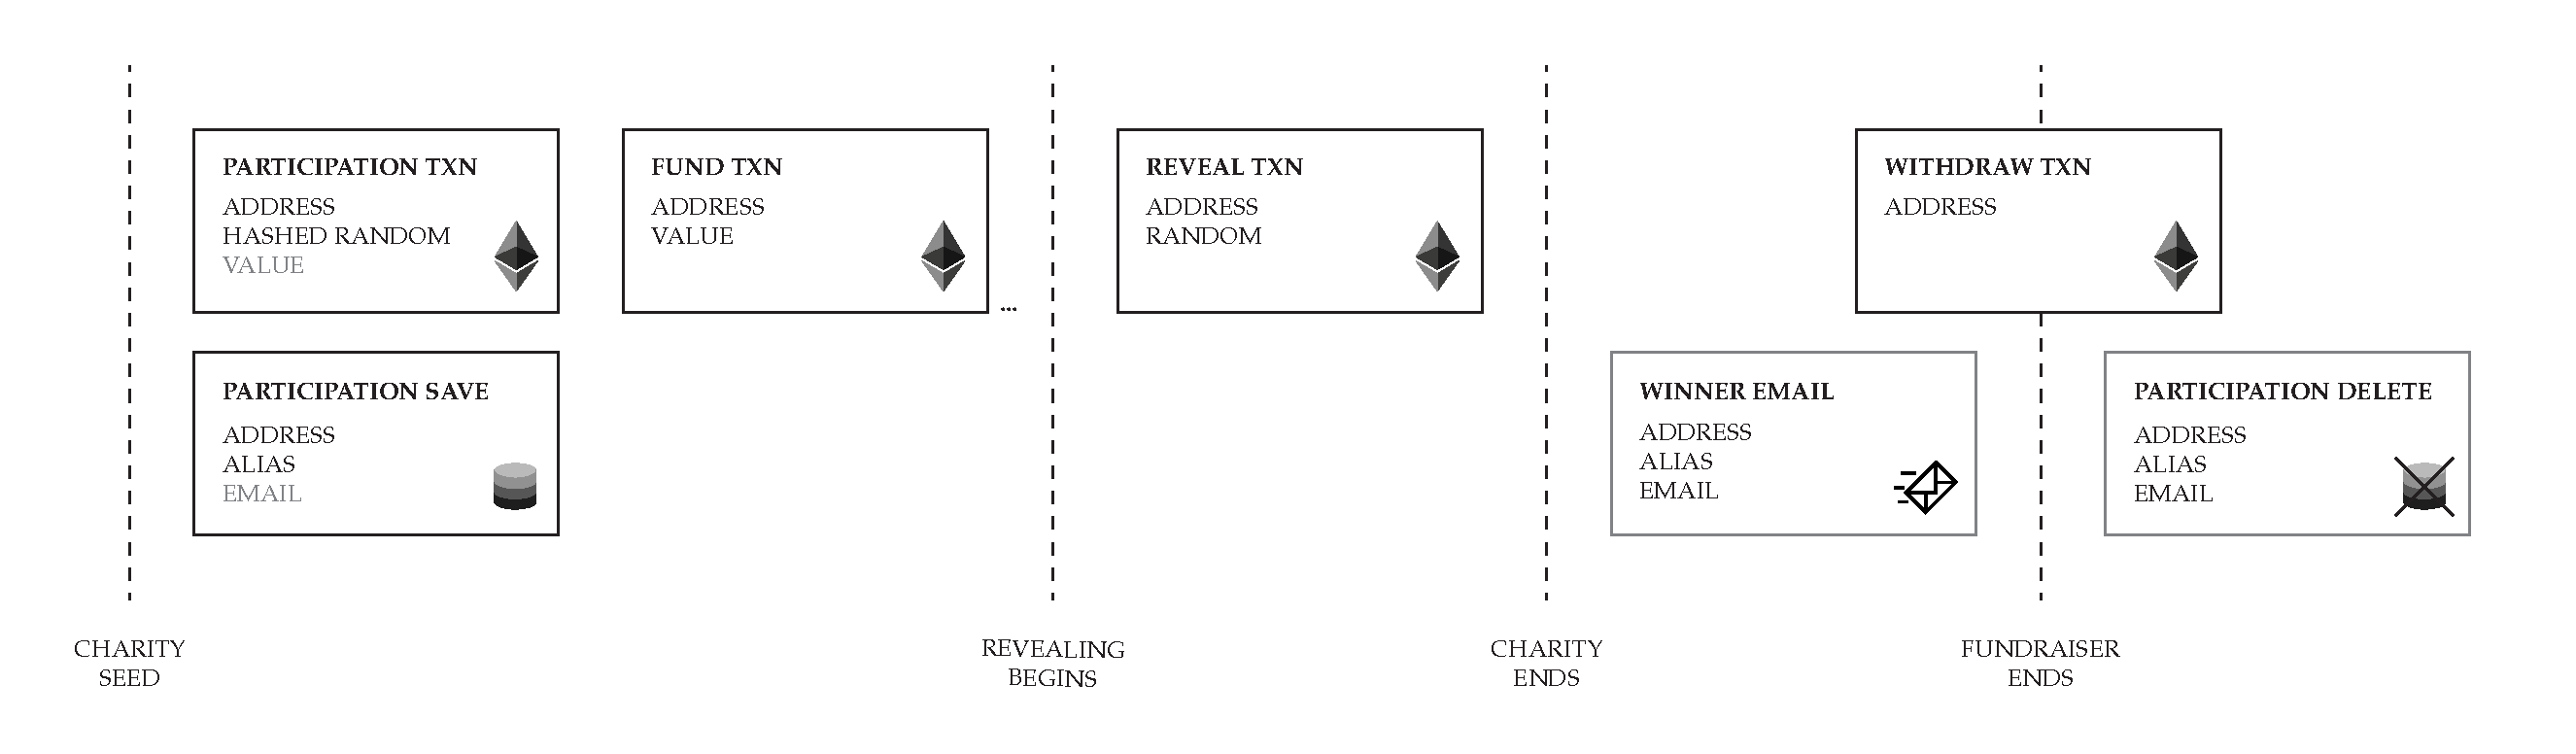
\includegraphics[width=1.0\textwidth]{participantDataFlow.pdf}
\caption{Participant data flow}
\label{figure:participantDataFlow}
\end{center}
\end{figure}

\subsection{Revelation Phase}

When the revelation phase begins, calls to the participate and fund functions will fail. Participants may now reveal their secret randoms, sent hashed in the participation phase, to the rest of the community. All of the hashed randoms need not be revealed; however, failing to reveal a random will result in the forfeiture of contributed funds and the ability to win through community selection. Successful revelation may only be performed once per participant and incorrect random revelations, determined using the formula in Figure \ref{figure:hashedRandomNumberFormula}, are rejected.

\subsection{Charity Ends}

When the revelation phase ends, participants are no longer allowed to reveal their randoms. Between the end time and expire time, both specified during kickoff, the charity must now reveal their random number provided during seed. If the charity fails to call the end function and reveal their random before the expire time, all entries are refundable through cancellation.

\subsubsection{Secure Deterministic Crowd-sourced Random Number Generation}

Because Ethereum is a Turing complete deterministic world computer, mining nodes cannot generate individual random numbers as they would never be able to reach consensus. Some decentralized applications decide to use a miner-defined value, such as the blockhash, timestamp, or other value to generate a random number. This technique is flawed given the miner's ability to ignore or reorder transactions and avoid broadcasting blocks entirely. It opens up the potential for the miner to receive additional chances of winning, even with deincentivization enhancements.

Seedom's method is similar to that of the RANDAO \cite{2}. It begins with a hashed random seed provided by the charity, a primary difference, the collection of secret hashed randoms in a participation phase and the revelation of these randoms during a revelation phase. All of the revealed random numbers are XORed together, beginning with all of the participant randoms and ending with the charity's random to produce a final universal crowd-sourced random used to determine the winning participant, as seen in figure \ref{figure:crowdsourcedRandomNumberGeneration}.

\begin{figure}[H]
\begin{center}
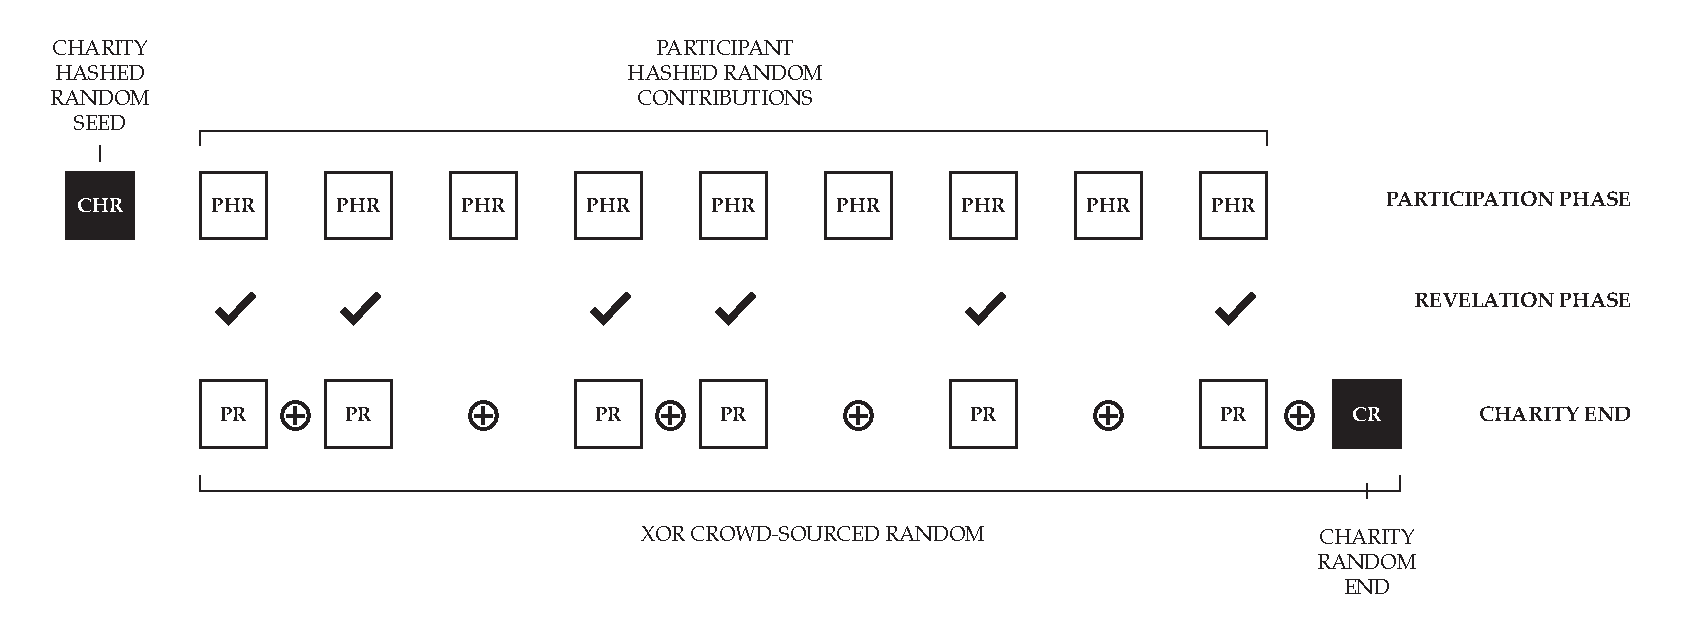
\includegraphics[width=1.0\textwidth]{crowdsourcedRandomNumberGeneration.pdf}
\caption{Crowd-sourced random number generation}
\label{figure:crowdsourcedRandomNumberGeneration}
\end{center}
\end{figure}

Due to miner transaction and block flexibility, the last participant always has a choice to reveal or not reveal their random before the end of the revelation phase. This option is only problematic if hashed randoms are collected and revealed solely from the participants as it gives each a double chance of winning. Worse, a miner that has participated many times using unique wallet addresses can gain many additional chances by reordering their reveal transactions and choosing which ones to publish. Because the cost of a Seedom entry will be low enough to be affordable by all, transaction gas and entry costs will not deincentivize maligned miners from using this method.

The charity must be used as a trusted third party to provide a final random number that can alter any manipulation by miners during the participation phase. Before the first supporter is allowed to participate, the charity must provide a hashed random number. This charity seed is required initially to prevent manipulation of the final crowd-sourced random by the charity itself. Users engaging in an ether-raiser tied to a specific charity are confirming their trust and support of the charity and their beneficial work by participation alone. This trust extends to the charity's ability to seed start the ether-raiser with their hashed random and end it with their final random revelation. The charity is incentivized to start and end an ether-raiser because of the funds they will receive.

\subsubsection{Winning Participant Selection}

After crowd-sourced random generation, but as part of the end call from the charity, the resulting number will be modded with the total number of revealed entries to determine an index into the global list of revealed entries. A discrete cumulative density function of entries is generated to assist with this process, and the participant associated with the entry at this index is the winning supporter. As the last step in this call, a map of balances updates with owed funds to the charity, winner, and owner. Ether is not immediately distributed to these wallets as to prevent invalid or malignant addresses from reverting the end function in the Ethereum Virtual Machine. The contract guarantees a winner during every bimonthly ether-raiser unless canceled.

After winning participant selection, but also as part of end call, a contract event will be broadcast that includes the participant's address, the participant's random number, and the total reward amounts calculated for the charity, winner, and Seedom. The participant's random, their alias, and their address serve as the pseudo-unique identifier of the winner.

\begin{figure}[H]
\begin{center}
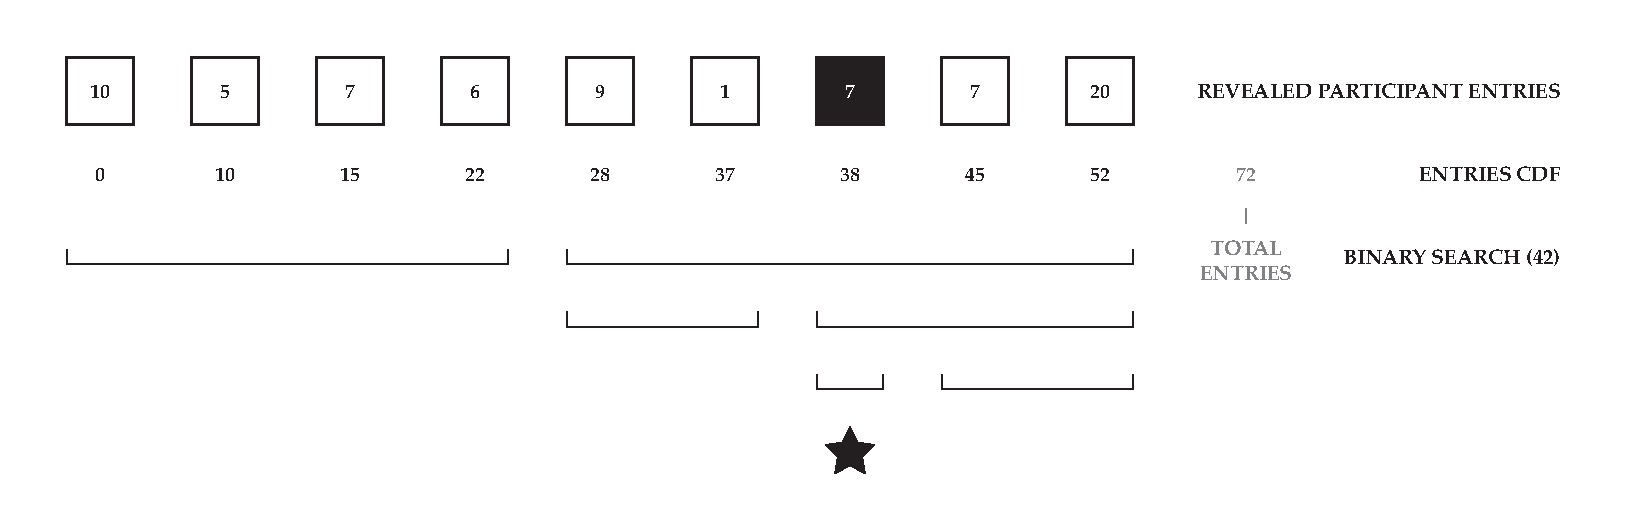
\includegraphics[width=1.0\textwidth]{winningParticipantSelection.pdf}
\caption{Winning participant selection for entry index 42}
\label{figure:winningParticipantSelection}
\end{center}
\end{figure}

\subsection{Ether-raiser Cancellation}

At any time after kickoff, but before charity seed, both the charity and the owner can cancel the ether-raiser. Cancellation is a simple process that refunds all participant entries obtained during the participation phase. The contract map of balances updates with these refunds. After the cancellation function is complete, users may withdraw their refunds using the withdraw function. Gas costs are non-refundable.

After the charity calls the end function, cancellation is impossible as the appropriation of funds in the map of balances is complete. However, if the charity fails to end a ether-raiser before the expiration time, the cancel function becomes open to the charity, the owner, and the entire community. This time-sensitive loophole ensures that every entry is refundable in the improbable event that something catastrophic happens to the owner, the charity, or both.

\section{Token Sale}
Never.

\section{Future Work}

In between ether-raiser, Seedom releases updates to our decentralized application as part of our continuous improvement process. If contract changes are involved, this will result in a new Seedom contract address for the next ether-raiser; however, due to the immutability of the blockchain and our lack of a self-destruct mechanism, legacy contracts will always be accessible for fund withdraws. The following are some of the improvements the Seedom team would like to implement.

\subsection{Efficient Participant Storage}

An order statistic tree \cite{5} will replace the dynamic participant storage array in the contract to facilitate future features of the application. The participants hash map remains the same, used in conjunction with this tree. A balanced and ordered statistic binary search tree allows for the efficient rank ordering of participant entries, and it is an essential step to providing support for a live participant leaderboard.

\subsubsection{Live Participants Leaderboard}

As more users participate, a live leaderboard will be available that tracks, in descending order, each participant's number of entries. If a user does not provide an alias during participation, their sending address is displayed. If the user does provide an alias, that instead. While not encouraged, participants are free to use this as a way of impromptu advertising. So if Company X wants their name to show on the Seedom homepage, they can buy the most entries to display themselves at the top of the leaderboard.

\subsection{Enhanced Random Number Generation Security}

Miner manipulation of the crowd-sourced random number generation process requires the Seedom team to adapt the random-generation algorithm in Figure \ref{figure:crowdsourcedRandomNumberGeneration} to stay ahead of potential security issues.

\subsubsection{Randomization of the Order of Participant Randoms}

In the first release, participant randoms considered in the crowd-sourced random number generation process are XORed in order of time of participation during the participation phase. Randomization of the order of the XORed randoms using the trusted charity's random as a seed would provide additional protection against last-minute miner manipulation of the final random.

\subsection{Handling Fund Growth}

As Seedom's participant base grows, our administration fee and winner selection process will evolve.

\subsubsection{Administration Fee Reduction}

The 5\% administration fee is adequate to maintain our decentralized application and protect the concept from any legal involvements that may arise. Many laws and organizations span the local and international jurisdictions that might impede the creation of a thoroughly transparent and trustless private global ether-raiser of this magnitude. As those concerns dwindle, our administration fee should follow in tandem, at our discretion, to ensure maximal returns to the charity and our community. Seedom's administration fee will never go above 5\%.

\subsubsection{Multiple Winning Participants}

There is an inherent burden that comes with a sizable influx of funds to any individual. Therefore, as the contribution fund grows immense, we may introduce, at our discretion, the ability for multiple winning participants. Each successive winner might receive more funds than the last one, or a pool of winners may equally split the ether. However, there will only be one benefiting charity for any ether-raiser.

\subsubsection{Physical Ether-raiser Phase}

After the end function completes, the charity, winning participant, and Seedom can now withdraw their funds by calling the withdraw function. These funds are available for withdrawing at any time and will never expire. As a best practice, Seedom recommends that everyone withdraw their funds as soon as possible.

Now that the ether-raiser is over, a physical fundraiser will take place near the headquarters of the benefiting charity to continue bringing awareness and contribution to their cause. This event will be open to the public, and everyone is welcome to attend. During the event, the Seedom team will assist the charity in their ability to accept direct ether donations and native fiat funds as well. Shortly after, the timeline will begin again with a different charity.

As the administration fund grows, the Seedom team will create a volunteer event during the physical fundraising phase to complement the charity ether-raiser. The winning participant or participants will be invited by email, if provided to Seedom, to an all-expenses-paid trip to both the volunteer and ether-raising events, wherever they may be in the world. Moreover, Seedom will send some of our team members along to assist the charity directly.

\subsection{Crowd-sourced Charity Selection}

After the first initial events, we will consider opening up the charity selection to a voting process. This will involve pre-selecting up to five charities that have expressed interest to work with Seedom and a one week voting period open to previous participants.

\section{Team Members}

The Seedom team is comprised of philanthropic entrepreneurs and enthusiasts from various sectors of the technology industry. The current employers of all team members have no affiliation with Seedom.

\vbox{
\begin{itemize}
\item{\href{https://www.linkedin.com/in/jesse-kuiper-cpa-771a2111}{Jesse Kuiper}, Founder \& President}
\item{\href{https://www.linkedin.com/in/awgneo}{Alex Groleau}, Founder \& Software Developer}
\item{\href{https://www.facebook.com/eric.l.m.thomas}{Eric Thomas}, Software Developer}
\item{\href{https://www.linkedin.com/in/kylegraden}{Kyle Graden}, Strategic Advisor}
\end{itemize}}

\pagebreak

\printbibliography

\vspace*{\fill}

\begin{flushright}

\pdfcreationdate
\end{flushright}
\end{document}